\newpage
\section{Ergebnisse und Berechnungen}
\label{sec:ergebnisse}
%Tabelle START
\begin{figure}[h!]
	\centering
	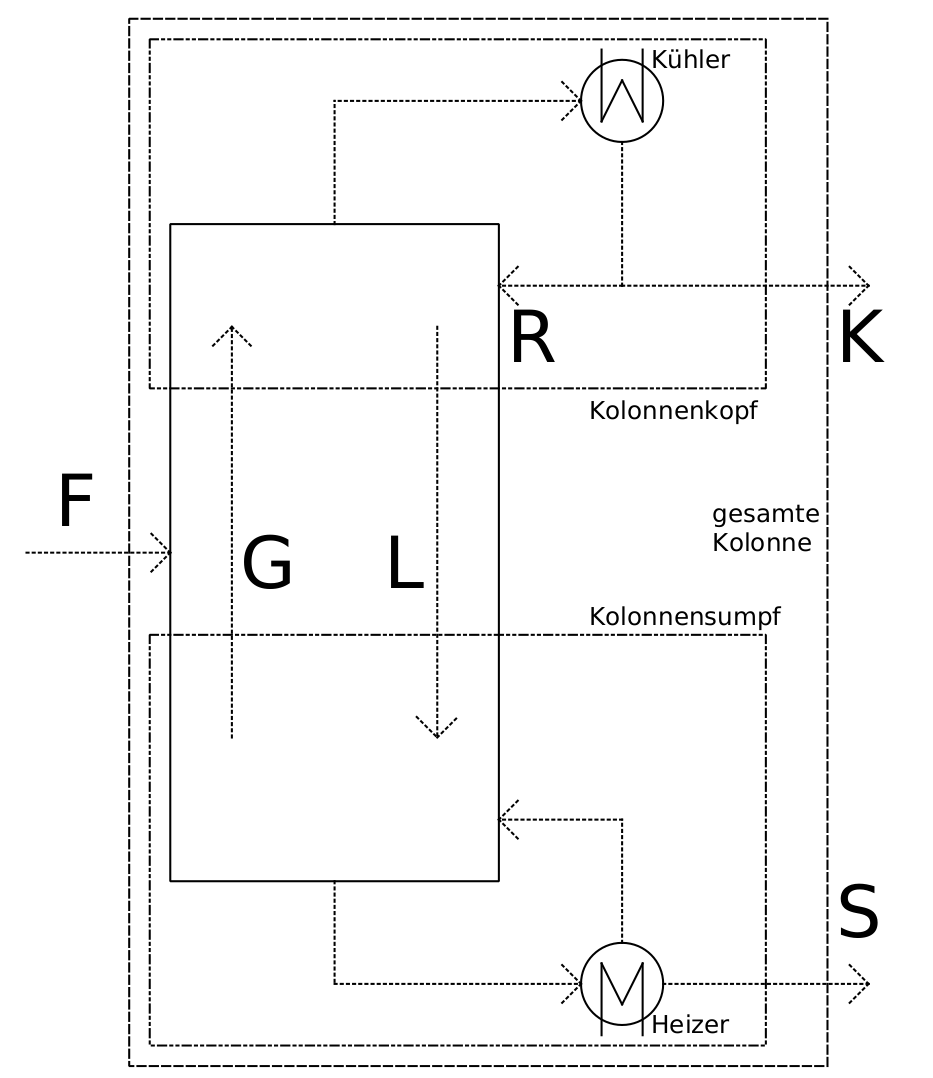
\includegraphics[width=0.7\linewidth]{img/Bilanzraumm}
	\caption{Schematische Abbildung der Rektifikationskolonne zur Darstellung der Bilanzräume}
	\label{fig:Bilanzraumm}
\end{figure}
\FloatBarrier
\subsection{Bilanzen}
\subsubsection{Gesamte Kolonne}

\hspace{5mm}\textbf{Gesamtstoffmengenbilanz}\\
\begin{equation}\label{gl:gesamtmolbilanzKOLONNE}
\dot{n}_F=\dot{n}_S+\dot{n}_K
\end{equation}

\hspace{5mm}\textbf{Komponentenbilanz - Ethanol} \\
\begin{equation}\label{gl:komponentenbilanzKOLONNE}
\dot{n}_F*x_{1F}=\dot{n}_S*x_{1F}+\dot{n}_K+x_{1K}
\end{equation}

\hspace{5mm}\textbf{Energiebilanz}\\
\begin{equation}\label{gl:energiebilanzKOLONNE}
\dot{H}_F+Q_{Heiz}=\dot{H}_K+\dot{H}_S+Q_{Kondensator}+Q_{Verlust}
\end{equation}


\subsubsection{Kolonnenkopf}

\hspace{5mm}\textbf{Gesamtstoffmengenbilanz}\\
\begin{equation}
\dot{n}_G=\dot{n}_L+\dot{n}_K
\end{equation}

\hspace{5mm}\textbf{Komponentenbilanz - Ethanol} \\
\begin{equation}
\dot{n}_G*y_{1}=\dot{n}_L*x_{1}+\dot{n}_K+x_{1K}
\end{equation}

\hspace{5mm}\textbf{Energiebilanz}\\
\begin{equation}
\dot{H}_G=\dot{H}_K+\dot{H}_L+Q_{Kondensator}+Q_{Verlust}
\end{equation}

\subsection{Berechnung der Zusammensetzung aus der Dichte}

Der Massenanteil an Ethanol der Proben wurde aus den gemessenen Dichten, durch einsetzen in eine Kalibrierfunktion berechnet. 
Die gegebene Kalibrierfunktion ist in Gleichung \eqref{gl:massenanteilausdichte} aufgeführt. 

\begin{equation}\label{gl:massenanteilausdichte}
	\rho \left[\si{\kg \per \raiseto{3}\meter}\right]=-0,0079826782*(w_1[\%])^2-1,2901290063*(w_1[\%])+998,2
\end{equation}
\subsection{Umrechnung von Massen- in Molenbruch}

Die zuvor erhaltenen Massenanteile werden nun, wie in Gleichung \eqref{gl:massINmol} gezeigt, in die entsprechenden Stoffmengenanteile umgerechnet.
\begin{flalign}\label{gl:massINmol}
	x_i&=\frac{\frac{w_i}{M_i}}{\sum\frac{w_j}{M_j}}\\
			x_1&=\frac{\frac{0,845}{\SI{46,07}{\gram\per\mole}}}{\frac{0,845}{\SI{46,07}{\gram\per\mole}}+\frac{1-0,845}{\SI{18,02}{\gram\per\mole}}}\\
			&=\underline{0,68}
\end{flalign}
\subsection{Berechnung des Molenstromes}

Die Berechnung des Molenstromes der Komponente 1 (Ethanol) an den betrachteten stellen wird analog der Beispielrechnung \eqref{gl:molenstrom} vorgenommen. Dabei werden die gemessene Dichte, der gemessene Volumenstrom, der berechnete Massenanteil und die Molare Masse der betrachteten Komponente eingesetzt.\\
\begin{flalign}\label{gl:molenstrom}
	\dot{n}&=\frac{\rho*\dot{V}*w}{M}\\
\dot{n}_{1K}	&=\frac{\rho_K*\dot{V}_K*w_{1K}}{M_1}\\
	&=\frac{\SI{832,3}{\kilogram\per\cubic\meter}*\SI{0,372}{\liter\per\hour}*0,845}{\SI{46,07}{\gram\per\mole}}\\
	&=\underline{\SI{5,67}{\mole\per\hour}}
\end{flalign}
Der gesamte Molenstrom an einer Stelle wird anschließend unter Zuhilfenahme des Molenbruchs der Komponente ausgerechnet.

\begin{flalign}
	\dot{n}_K&=\frac{\dot{n}_{1K}}{x_{1K}}\\
	&=\frac{\SI{5,67}{\mole\per\hour}}{0,68}\\
	&=\underline{\SI{8,34}{\mole\per\hour}}
\end{flalign}
\subsection{Berechnung des Molenstromes im Sumpf}

Aus den Bilanzgleichungen \eqref{gl:gesamtmolbilanzKOLONNE} und \eqref{gl:komponentenbilanzKOLONNE} ergibt sich ein überbestimmtes Gleichungssystem. Die Berechnung des Molenstromes im Sumpf der Kolonne erfolgt durch Anwendung des Excel-Add-Ins \emph{solver}. Der Feed-Molenstrom wird aufgrund der größten Fehleranfälligkeit als veränderliche Größe markiert. Nebenbedingung für die Lösung ist, dass  \eqref{gl:gesamtmolbilanzKOLONNE} und \eqref{gl:komponentenbilanzKOLONNE} den selben Wert annehmen. Für die Daten des ersten Versuches folgt ein Sumpf-Molenstrom von \SI{227,27}{\mole\per\hour}. Der Feed-Molenstrom wird durch die Anwendung von ursprünglich \SI{225,39}{\mole\per\hour} auf \SI{235,60}{\mole\per\hour} angehoben. 


\subsection{Rücklaufverhältnis}
Bei einem stationären Betrieb der Rektifikationskolonne im thermischen Gleichgewicht ist auch der Volumenstrom am Kopfprodukt stationär. Daher können für das Rücklaufverhältnis auch die Zeiten eingesetzt werden, in welchen das Magnetventil den jeweiligen Weg freigibt. Dabei wurde die, sich auf dem Verschlussstopfen gesammelte, Flüssigkeitspfütze berücksichtigt.

\begin{equation}
	\nu=\frac{\dot{R}}{\dot{E}}=\frac{t_{\dot{R}}}{t_{\dot{E}}}=\frac{\SI{11,01}{\second}}{\SI{3,99}{\second}}=\underline{2,76}
\end{equation}

\subsection{McCabe-Thiele-Diagramm}
Nachdem die Ethanolanteile von Kopfprodukt, Feed und Sumpfprodukt als senkrechte Linien in das Gleichgewichtsdiagramm eingetragen sind, kann die Arbeitsgerade des Verstärkungsteils aus dem Punkt $y_o$(vgl.\eqref{gl:yo}) und dem Schnittpunkt von Diagonale und senkrechter auf $x_K$ durch Verbinden der beiden Punkte konstruiert werden. Die Abtriebsgerade folgt aus dem Schnittpunkt der Senkrechten über $x_F$ und der Verstärkungsgerade und dem Schnittpunkt der senkrechten über $x_S$ mit der Diagonalen. Die Stufenkonstruktion erfolgt ausgehend vom Schnittpunkt von Diagonale und senkrechter auf $x_K$, bis zum überschreiten des Schnittpunktes von Diagonale und senkrechter auf $x_S$. Die fertige Stufenkonstruktion ist in Abb. \ref{fig:McCabe} dargestellt. Es ergaben sich 6 theoretische Trennstufen. Diese Anzahl liegt weit unter der wirklichen Bodenzahl von 15. 

\begin{flalign}\label{gl:yo}
	y_o&=\frac{x_K}{\nu+1}\\
	&= \frac{x_K}{\nu+1}=\frac{0,68}{2,76+1}=\underline{0,181}
\end{flalign}
\vspace{-2mm}
\begin{figure}[h!]
	\centering
	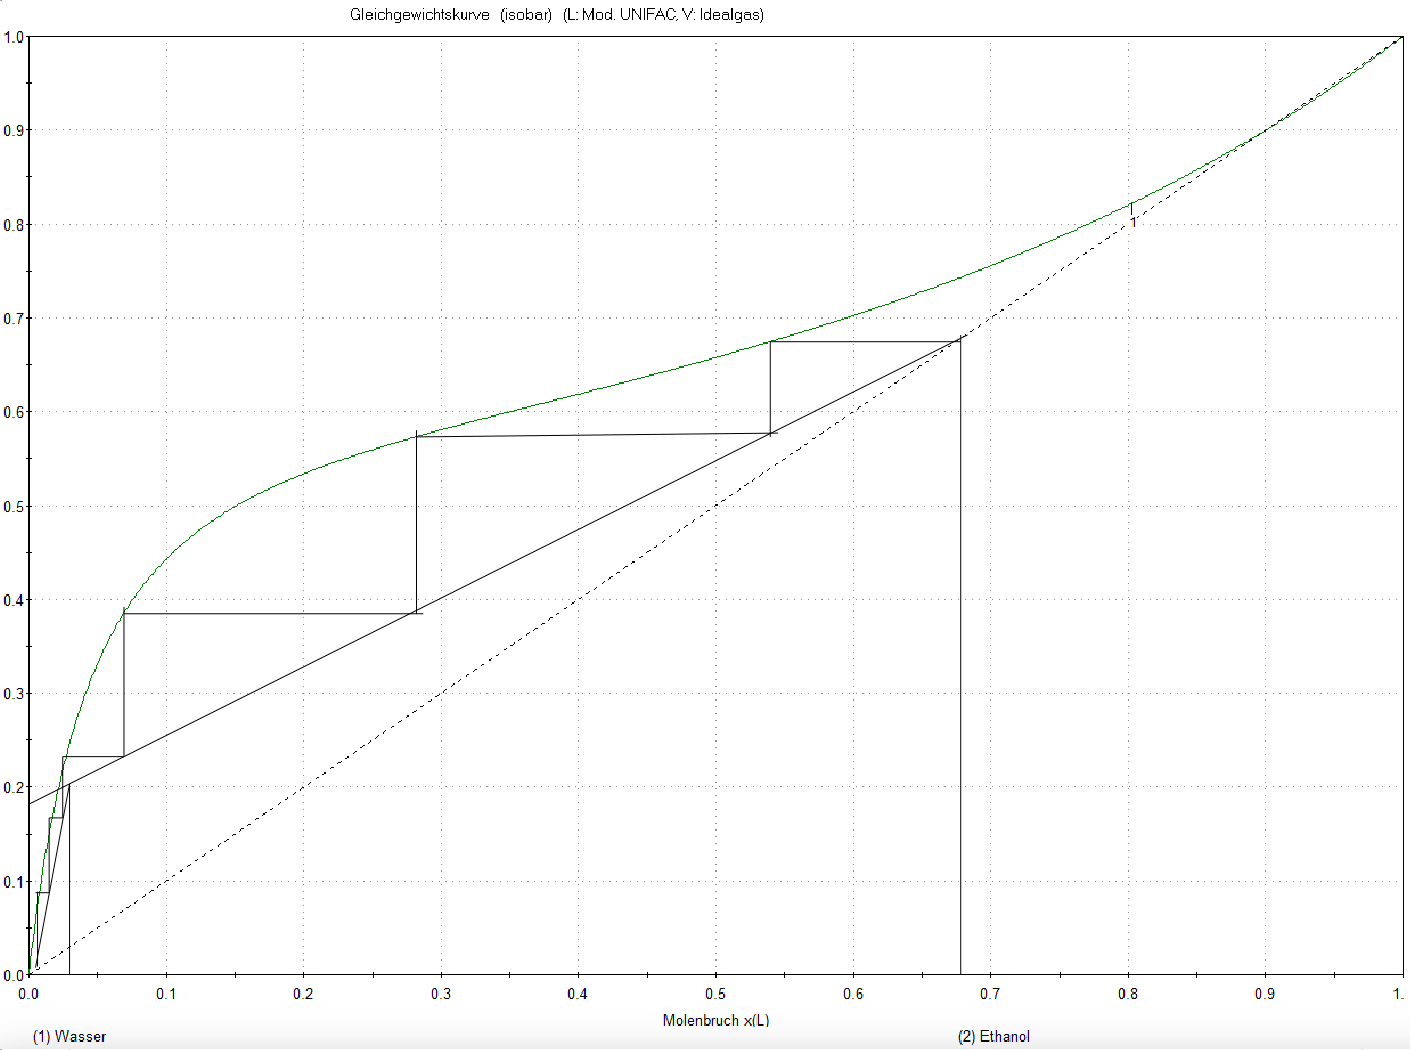
\includegraphics[width=0.85\linewidth]{img/McCabe}
	\caption{Das Gleichgewichtsdiagramm des Versuch 1 mit der resultierenden Stufenkonstruktion - von Hand}
	\label{fig:McCabe}
\end{figure}
\FloatBarrier
\begin{figure}[h!]
	\centering
	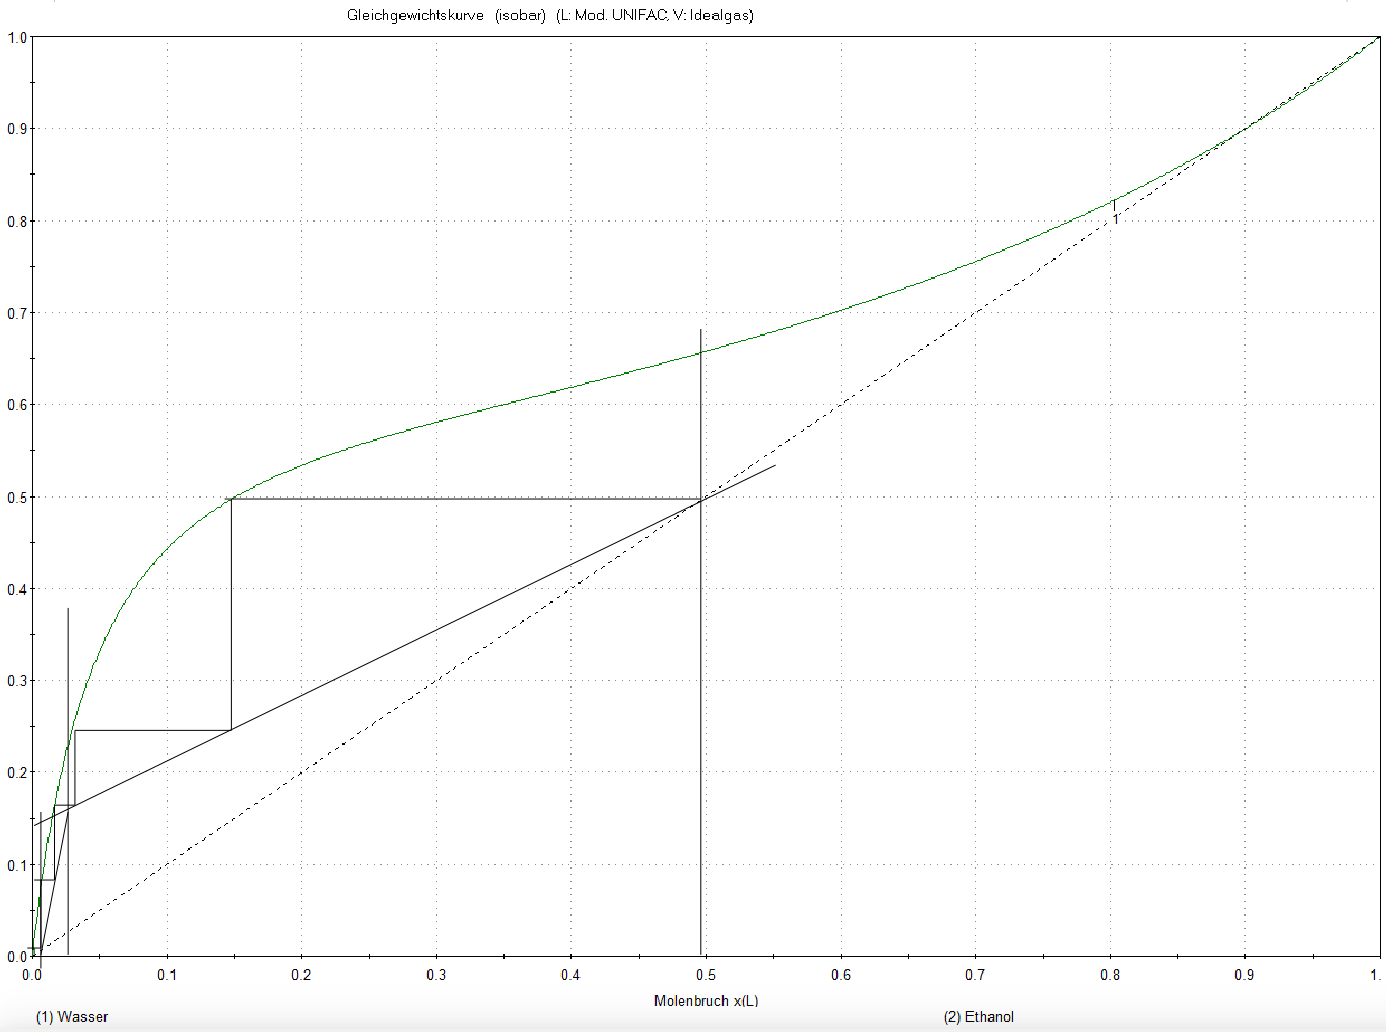
\includegraphics[width=0.85\linewidth]{img/McCabe2(5Stufen)}
	\caption{Das Gleichgewichtsdiagramm des Versuch 2 mit der resultierenden Stufenkonstruktion - von Hand}
	\label{fig:McCabe2}
\end{figure}
\FloatBarrier

\begin{figure}[h!]
	\centering
	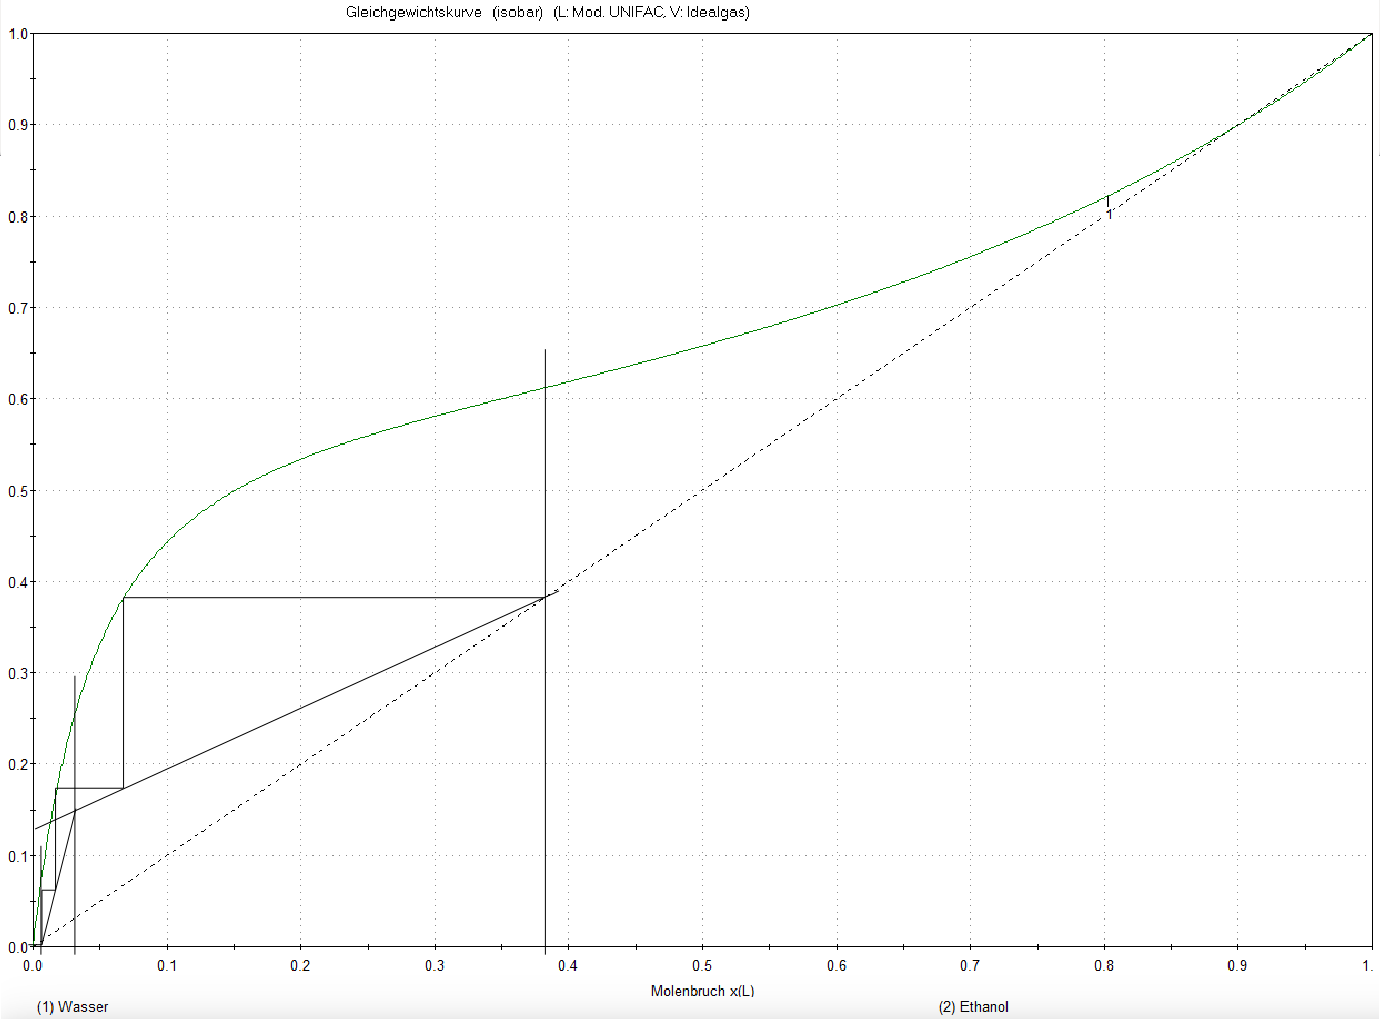
\includegraphics[width=0.85\linewidth]{img/McCabe3(4Stufen)}
	\caption{Das Gleichgewichtsdiagramm des Versuch 3 mit der resultierenden Stufenkonstruktion - von Hand}
	\label{fig:McCabe3}
\end{figure}
\FloatBarrier

\begin{figure}[h!]
	\centering
	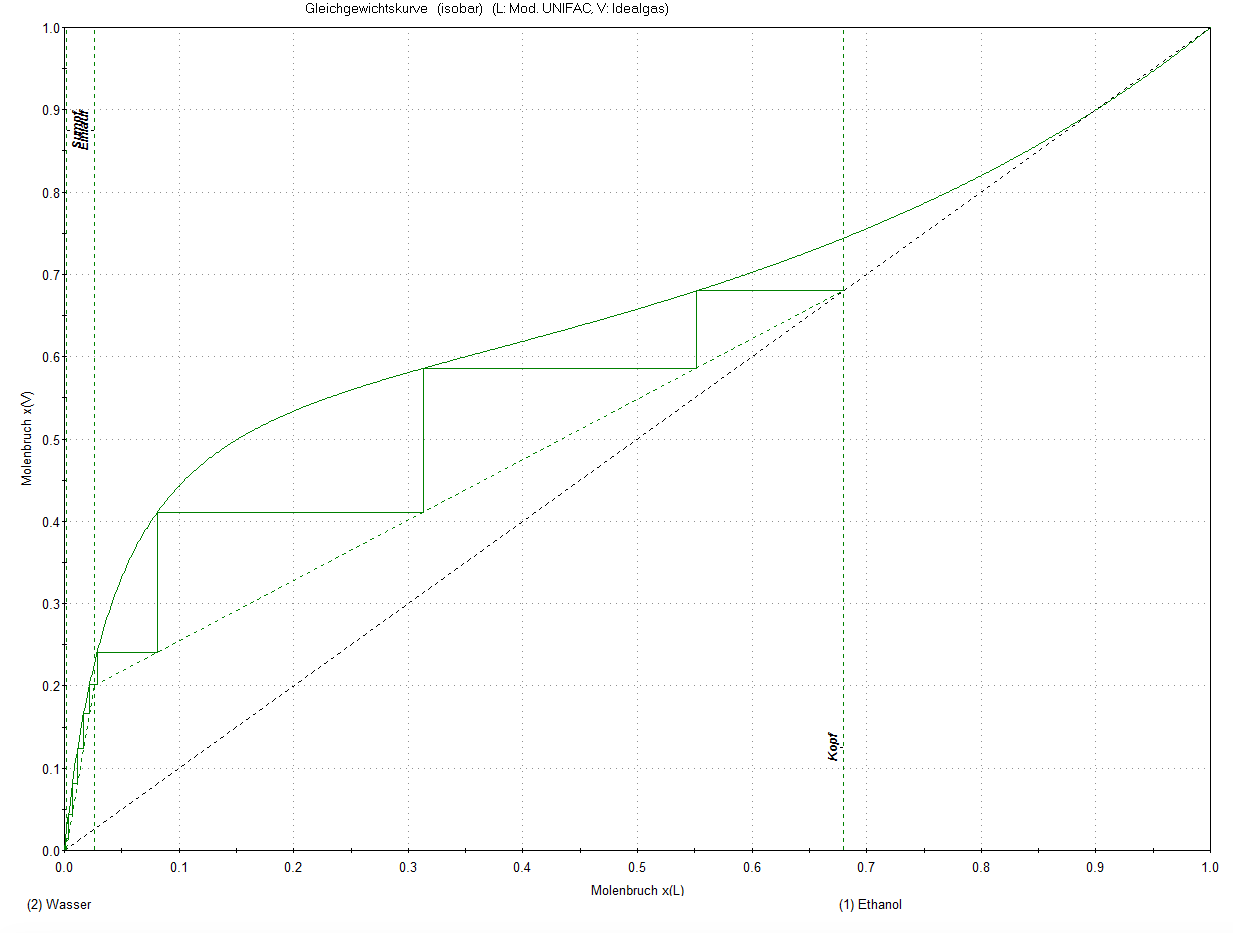
\includegraphics[width=0.85\linewidth]{img/VLE-MC-1}
	\caption{Das Gleichgewichtsdiagramm des Versuch 1 mit der resultierenden Stufenkonstruktion - automatisch}
	\label{fig:versuchsaufbau-ebull}
\end{figure}
\FloatBarrier
\begin{figure}[h!]
	\centering
	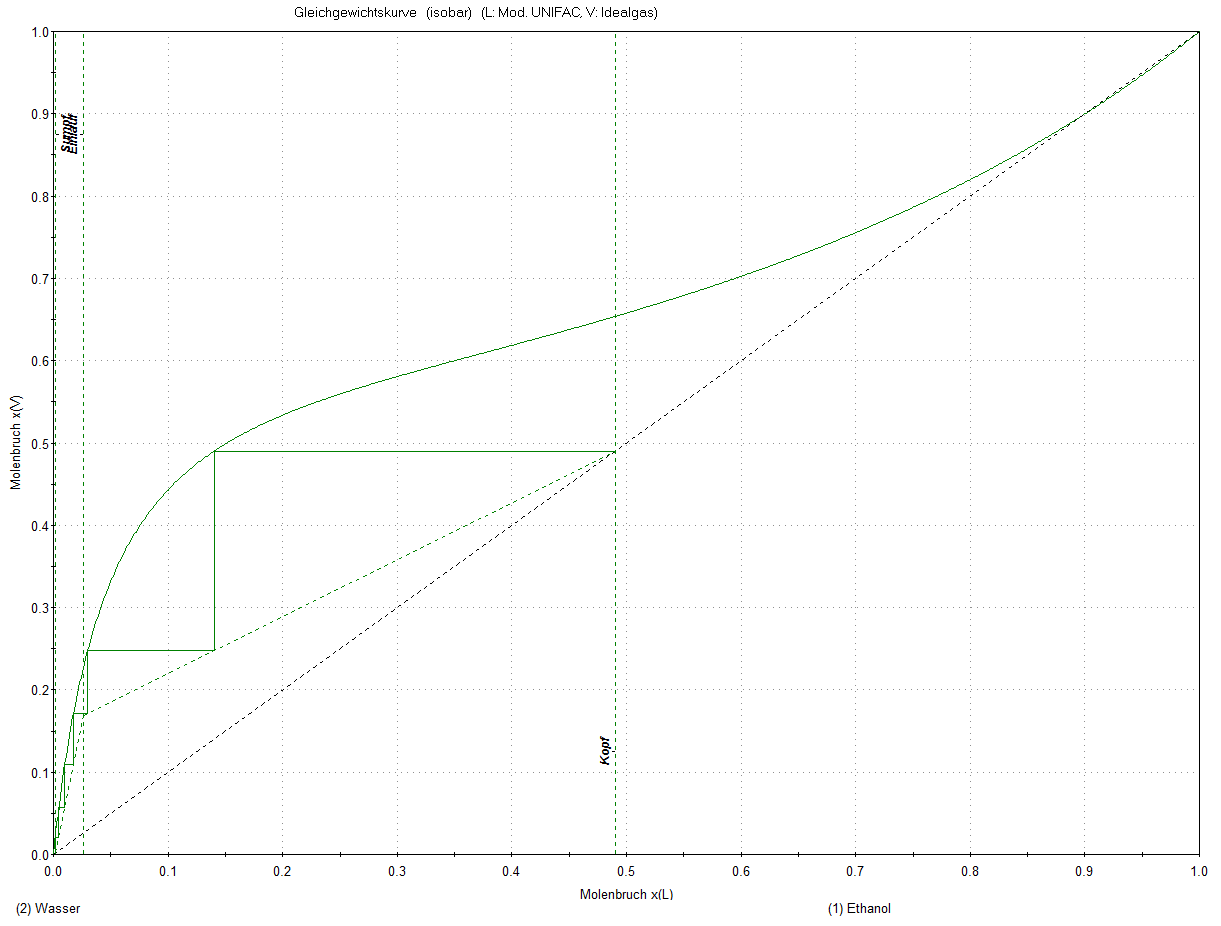
\includegraphics[width=0.85\linewidth]{img/VLE-Mc-2}
	\caption{Das Gleichgewichtsdiagramm des Versuch 2 mit der resultierenden Stufenkonstruktion - automatisch}
	\label{fig:versuchsaufbau-ebull}
\end{figure}
\FloatBarrier
\begin{figure}[h!]
	\centering
	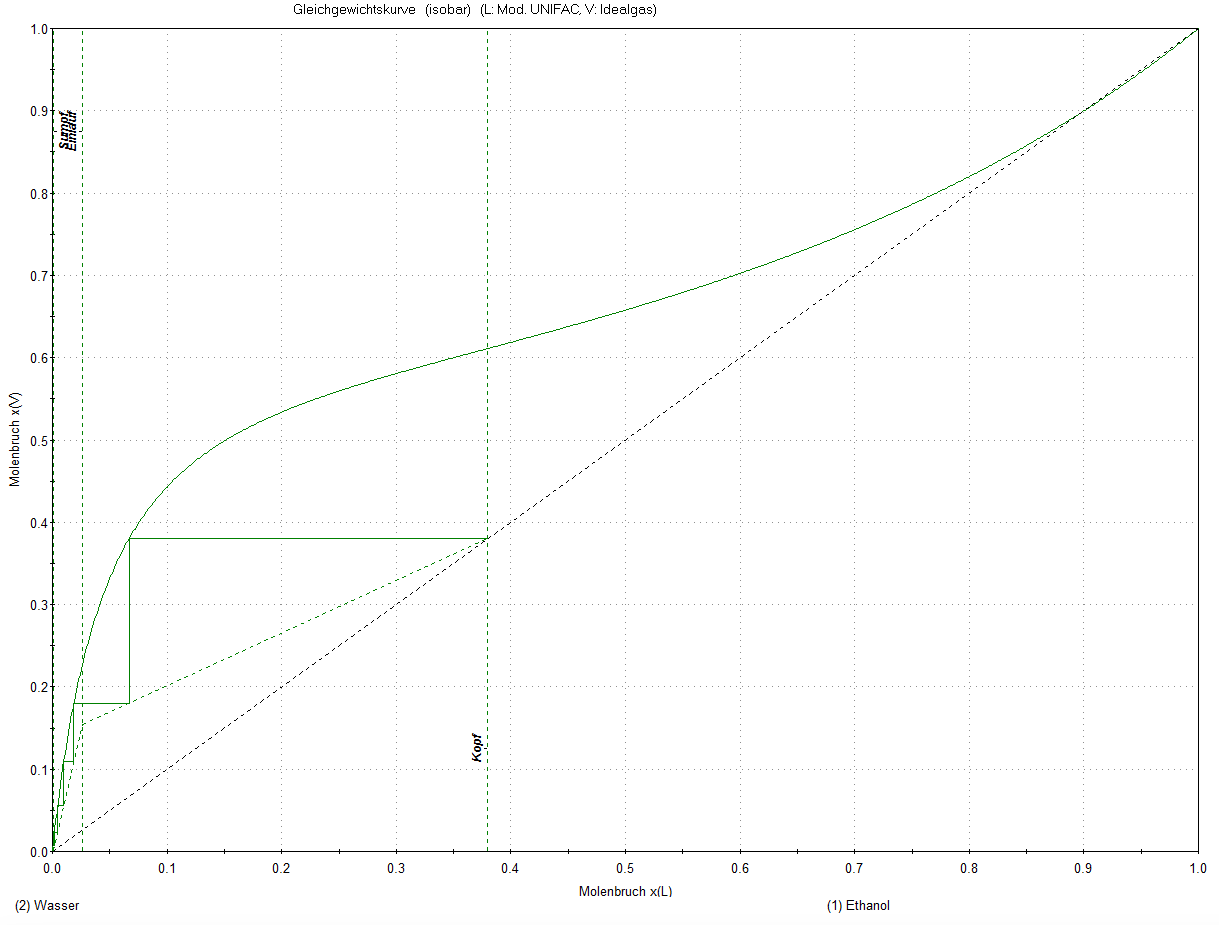
\includegraphics[width=0.85\linewidth]{img/VLE-Mc-3}
	\caption{Das Gleichgewichtsdiagramm des Versuch 3 mit der resultierenden Stufenkonstruktion - automatisch}
	\label{fig:versuchsaufbau-ebull}
\end{figure}
\FloatBarrier




\subsection{Energiebilanz}
Um in die Gleichung \eqref{gl:energiebilanzKOLONNE} als Energiebilanz einsetzen zu können, müssen zuerst die Enthalpien der Ströme berechnet werden. Für diese wiederum ist die spezifische Wärmekapazität erforderlich. Außerdem muss die Kühl und Heizleistung bekannt sein. Die Berechnungen sind in den nachfolgenden Abschnitten detailliert aufgeführt. Die Gleichung \eqref{gl:Energie-eingesetzt} enthält die eingesetzten Zwischenergebnisse. Durch diese Energiebilanz lässt sich die Verlustwärme berechnen. Diese beträgt im ersten Versuch \SI{637,5}{\watt}.
\begin{flalign}\label{gl:Energie-eingesetzt}
\dot{H}_F+Q_{Heiz}&=\dot{H}_K+\dot{H}_S+Q_{Kondensator}+Q_{Verlust}\\
	\SI{108,29}{\watt}+\SI{1229,36}{\watt}&=\SI{21,66}{\watt}+\SI{475,94}{\watt}+\SI{202,55}{\watt}+Q_{Verlust}\\
	Q_{Verlust}&=\underline{\SI{637,5}{\watt}}
\end{flalign}

\subsubsection{Wärmekapazitäten}
Die Wärmekapazitäten der Mischungen, werden durch Wichtung der Wärmekapazitäten der Reinstoffe, bei der gemessenen Temperatur, mit den Molenbrüchen, nach Gleichung \eqref{gl:cp} berechnet. Die Wärmekapazität der Reinstoffe ist durch dir Regressionsgleichung \eqref{gl:regCP} und die tabellierten Konstanten A, B, C, D und E gegeben.
\begin{equation}\label{gl:regCP}
	cp\,\, \left[\SI{}{\joule\per\kilo\mole\per\kelvin}\right]=A+B*T+C*T^2+D*T^3+E*T^4
\end{equation}
\begin{flalign}\label{gl:cp}
	\bar{c_p}(K)&=x_1*c_{p1}+x_2*c_{p2}\\
	&=0,68*\SI{138673}{\joule\per\kilo\mole\per\kelvin}+(1-0,68)*\SI{75569}{\joule\per\kilo\mole\per\kelvin}\\
	&=\underline{\SI{118481,84}{\joule\per\kilo\mole\per\kelvin}}
\end{flalign}

\subsubsection{Enthalpien der Ströme}

\begin{flalign}
	\dot{H}&=\dot{n}*cp*\Delta T\\
	\dot{H}_K&=\dot{n}_K*c_{pK}*\Delta T_K\\
	&=\SI{8,34}{\mole\per\hour}*\SI{118481,84}{\joule\per\kilo\mole\per\kelvin}*\SI{78,9}{\kelvin}\\
	&=\underline{\SI{21,66}{\watt}}\\%===================
	\dot{H}_F&=\dot{n}_F*c_{pF}*\Delta T_F\\
	&=\SI{236,995}{\mole\per\hour}*\SI{76386,75}{\joule\per\kilo\mole\per\kelvin}*\SI{21,65}{\kelvin}\\
	&=\underline{\SI{108,29}{\watt}}\\
		\dot{H}_S&=\dot{n}_S*c_{pS}*\Delta T_S\\
		&=\SI{227,27}{\mole\per\hour}*\SI{76112,46}{\joule\per\kilo\mole\per\kelvin}*\SI{99,05}{\kelvin}\\
		&=\underline{\SI{475,94}{\watt}}\\
\end{flalign}
\subsubsection{Kühlleistung}

\begin{flalign}
	\dot{Q}&=\dot{m}*c_p*\Delta T\\
	&=\rho*\dot{V}*c_p*(T_\omega-T_\alpha)\\
	&=\SI{999,38}{\kilogram\per\cubic\meter}*\SI{28,25e-3}{\cubic\meter\per\hour}*\SI{4200}{\joule\per\kilogram\per\kelvin}*(\SI{19,45}{\degreeCelsius}-\SI{13,3}{\degreeCelsius})*\si{\kelvin}\\
	&=\underline{\SI{202,55}{\watt}}
\end{flalign}
\subsubsection{Berechnung der Heizleistung}

Die Berechnung der Heizleistung in Watt beruht auf der verbrauchten Energie über einen gewissen Zeitraum. Definitionsgemäß kann daher die Heizleistung entsprechend der nachfolgenden Gleichung \eqref{gl:Qheizung} berechnet werden.

\begin{flalign}\label{gl:Qheizung}
\dot{Q}_{Heizung}&=\frac{Q_{Heizung}[W*h]}{t[s]/3600}\\
&=\frac{\SI{358,3}{\watt\hour}}{\SI{1049}{\second}/3600}\\
&=\underline{\SI{1229,36}{\watt}}
\end{flalign}